\documentclass{article}

% Bibliography
\usepackage{natbib}
\bibpunct{(}{)}{;}{a}{}{;}

% Use 'It was found that A is B (Name 1234)' style
\setcitestyle{authoryear,open={},close={}}

% Affiliations
\usepackage{authblk}
\title{babette: BEAUti 2, BEAST2 and Tracer for R}
\author[1]{Rich\`el J.C. Bilderbeek}
\author[1]{Rampal S. Etienne}
\affil[1]{Groningen Institute for Evolutionary Life Sciences, University of Groningen, Groningen, The Netherlands}

% Use double spacing
\usepackage{setspace}
\doublespacing

\usepackage{listings}
\usepackage{hyperref}
\usepackage{todonotes}
\usepackage{verbatim}
\usepackage{tikz}
\usepackage{tkz-graph}
\usepackage{pgf}
\usepackage{bm}

\usetikzlibrary{arrows,automata}

% Style of listings
% From http://r.789695.n4.nabble.com/How-to-nicely-display-R-code-with-the-LaTeX-package-listings-tp4648110.html
\usepackage{fancyvrb} 
\definecolor{codegreen}{rgb}{0,0.6,0}
\definecolor{codegray}{rgb}{0.5,0.5,0.5}
\definecolor{codepurple}{rgb}{0.58,0,0.82}
\definecolor{backcolor}{rgb}{0.95,0.95,0.92}
\lstdefinestyle{mystyle}{
  language=R,% set programming language
  basicstyle=\ttfamily\small,% basic font style
  commentstyle=\color{gray},% comment style
  % numbers=left,% display line numbers on the left side
  numberstyle=\scriptsize,% use small line numbers
  numbersep=10pt,% space between line numbers and code
  tabsize=2,% sizes of tabs
  showstringspaces=false,% do not replace spaces in strings by a certain character
  captionpos=b,% positioning of the caption below
  breaklines=true,% automatic line breaking
  escapeinside={(*}{*)},% escaping to LaTeX
  fancyvrb=true,% verbatim code is typset by listings
  extendedchars=false,% prohibit extended chars (chars of codes 128--255)
  alsoletter={.<-},% becomes a letter
  alsoother={$},% becomes other
  otherkeywords={!=, ~, $, \&, \%/\%, \%*\%, \%\%, <-, <<-, /},% other keywords
  deletekeywords={c}% remove keywords 
}
\lstset{style=mystyle}

% Adds numbered lines
\usepackage{lineno}
\linenumbers

% Rename 'Abstract' to 'Summary 
\usepackage[english]{babel}
\addto{\captionsenglish}{\renewcommand{\abstractname}{Summary}}

\usetikzlibrary{calc}
\usetikzlibrary{arrows.meta}

\begin{document}

\maketitle

%%%%%%%%%%%%%%%%%%%%%%%%%%%%%%%%%%%%%%%%%%%%%%%%%%%%%%%%%%%%%%%%%%%%%%%%%%%%%%%%%%%%%%
% Figures at the end
%%%%%%%%%%%%%%%%%%%%%%%%%%%%%%%%%%%%%%%%%%%%%%%%%%%%%%%%%%%%%%%%%%%%%%%%%%%%%%%%
\begin{figure}[h]
  \centering
  \resizebox {0.8\columnwidth} {!} {
    \begin{tikzpicture}[->,>=stealth',shorten >=1pt,auto,node distance=6cm, semithick]   
    \tikzstyle{every state}=[]
    \node[state] (A) [rectangle] {
      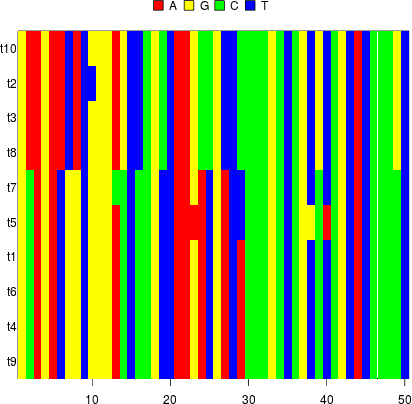
\includegraphics[width=0.2\textwidth]{alignment.png}
    };   
    \node[state] (AL) [above left=-0.25cm and -0.25cm of A, fill=white] {
      1
    };   
    \node[state] (B) [right of = A, rectangle] {
      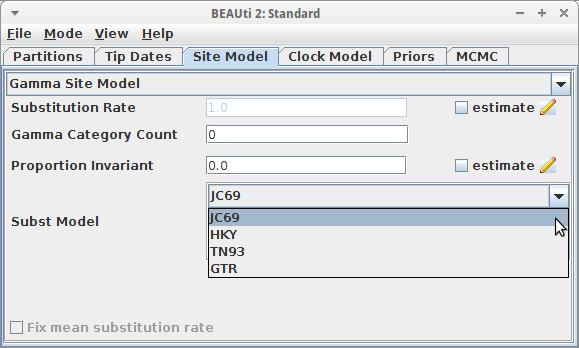
\includegraphics[height=0.15\textheight]{BeautiSiteModel.png}
    };   
    \node[state] (BL) [above left=-0.25cm and -0.25cm of B, fill=white] {
      2
    };   
    \node[state] (E) [below of=A, rectangle] {
      
\includegraphics[height=0.1\textheight]{file2.png}
    };   
    \node[state] (EL) [above left=-0.25cm and -0.25cm of E, fill=white] {
      3
    };   
    \node[state] (C) [right of = E, rectangle] {
      
\includegraphics[width=0.3\textwidth]{beast_logo.png}
    };   
    \node[state] (CL) [above left=-0.25cm and -0.25cm of C, fill=white] {
      4
    };   
    \node[state] (F) [rectangle, below of=E] {
      
\includegraphics[height=0.1\textheight]{file.png}
    };
    \node[state] (FL) [above left=-0.25cm and -0.25cm of F, fill=white] {
      5
    };   
    \node[state] (H) [rectangle, below of=F] {
      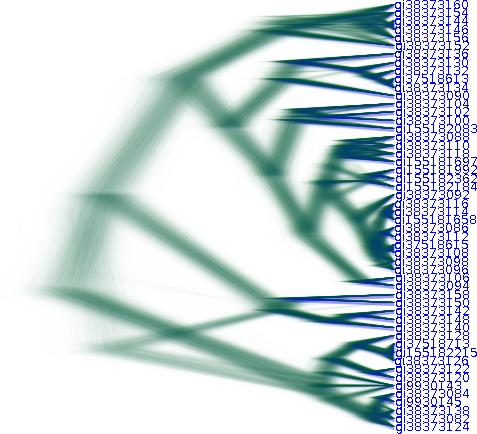
\includegraphics[width=0.3\textwidth]{DensiTreeExample2.jpg}
    };
    \node[state] (HL) [above left=-0.25cm and -0.25cm of H, fill=white] {
      6
    };   
    \node[state] (I) [rectangle, right of=H] {
      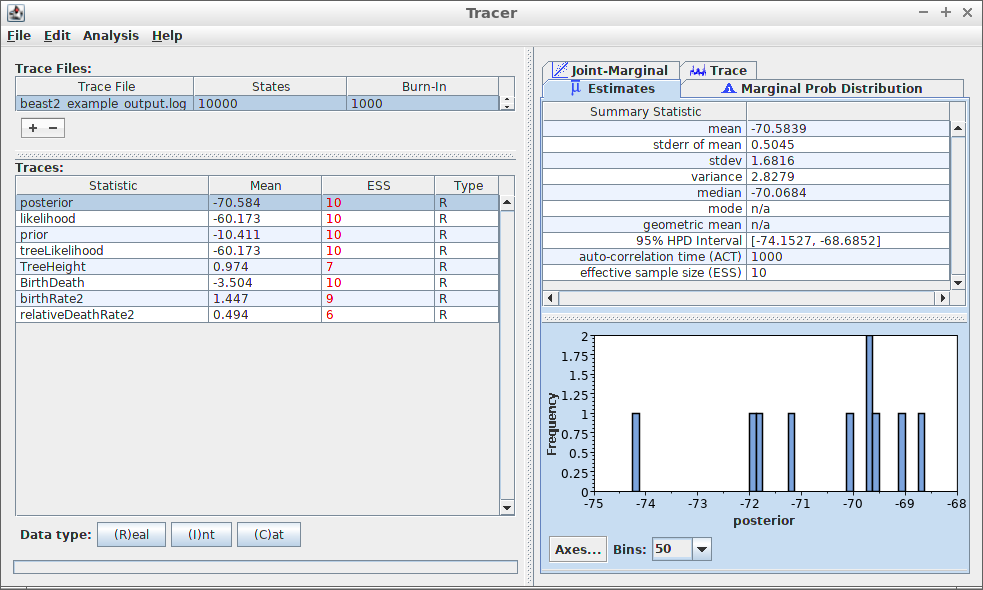
\includegraphics[width=0.6\textwidth]{tracer_example_output.png}
    };
    \node[state] (IL) [above left=-0.25cm and -0.25cm of I, fill=white] {
      7
    };   
    \path 
      (A) edge [anchor = west] node {} (E)
      (E) edge [anchor = west] node {} (F)
      (F) edge [anchor = west] node {} (H)
      (F) edge [anchor = west] node {} (I)
    ; 
    \path [-o,draw] (B) -- ($ (A) !.5! (E) $);
    \path [-o,draw] (C) -- ($ (E) !.5! (F) $);
    \end{tikzpicture}
  }
  \caption{
    Workflow using GUI tools. From an alignment (1) and BEAUti (2), 
    a BEAST2 configuration file (3) is created. BEAST2 (4) uses that file
    to infer a posterior, storing it in multiple files (5). These results
    are visualized using DensiTree (6) and Tracer (7). babette allows
    for the same workflow, all from an R function call.
  }
  \label{fig:workflow}
\end{figure}
%%%%%%%%%%%%%%%%%%%%%%%%%%%%%%%%%%%%%%%%%%%%%%%%%%%%%%%%%%%%%%%%%%%%%%%%%%%%%%%%

\end{document}
